\documentclass[conference]{IEEEtran}
\usepackage[T1]{fontenc}
\usepackage{amsmath,amssymb}
\usepackage{graphicx}
\usepackage{booktabs}
\usepackage{cite}
\usepackage{url}
\usepackage{microtype}
\usepackage[hidelinks]{hyperref}
\newtheorem{proposition}{Proposition}
\newenvironment{proof}{\begin{IEEEproof}}{\end{IEEEproof}}
\graphicspath{{figures/}}
\begin{document}
\title{Cyber-Resilient Recovery of Electric Vehicle\\Charging Under Uncertain Command Execution}
\author{\IEEEauthorblockN{Ali Sayghe and Ahmed Sultan}
\IEEEauthorblockA{Department of Electrical and Electronic Engineering\\
Yanbu Industrial College, Royal Commission for Jubail and Yanbu\\
Yanbu, Saudi Arabia\\
sayghea@rcjy.edu.sa, Sultanba@rcjy.edu.sa}}
\maketitle
\begin{abstract}
Uncertain execution of electric vehicle charging commands can invalidate feeder
capacity reallocation during recovery. We reserve capacity for charging caps
consistent with causal execution evidence, including unresolved commands and
expiry fallback. A trusted adapter supplies generation fencing, absolute expiry,
and post-application certificates. A conditional proposition establishes cap
containment and feasibility of selected affine network constraints. Nonlinear
power-flow replay evaluates 3,980 episodes on IEEE 123-node and 13-node feeders
with synthetic requests. Serialized and nonexpanding-supersession ledger variants
exhibit no electrical violations in their evaluated cases. In the main impaired
cases, supersession delivers 26.3\% more energy than static quotas; a tuned feedback
baseline violates limits in 22 of 240 cases. Supersession delivers 0.51\% less
energy than serialization, with a paired 95\% interval of \textminus3.23 to
\textminus1.69~kWh. A separately specified retry follow-up on new cohorts narrows
this deficit to 0.17\%. Field validation remains future work.

\end{abstract}
\begin{IEEEkeywords}
Capacity reservation, charging recovery, cyber-physical security,
distribution networks, electric vehicles.
\end{IEEEkeywords}
\section{Introduction}
\label{sec:introduction}
Recovery of coordinated electric vehicle (EV) charging requires knowing which
power limits can still execute. If a requested reduction is delayed, reallocating
its capacity elsewhere can overload the feeder. A later measurement of low draw
also need not exclude an unresolved increase or a higher fallback after profile
expiry. These ambiguities concern executable limits as well as communication
availability and charging demand.

For example, a 10-kW shared limit and active caps $(8,2)$ cannot support
reallocation to $(2,8)$ until the first reduction is established. If a temporary
2-kW profile later expires to an 8-kW fallback, the same risk returns even after
the reduction was observed. Recovery must account for both transitions.

Timed Command Interference links delayed commands and timeout fallback to EV
scheduling violations; its proposed future defenses include execution
verification and resilient coordination \cite{marandi2026tci}.
Related resilience mechanisms include capacity sharing
during communication outages \cite{gumrukcu2024dcs}, feedback scheduling under
uncertain charge acceptance \cite{kandpal2022feedback}, and distributed recovery
from corrupted scheduling messages \cite{qu2026resilient}. Networked predictive
control already addresses uncertain applied inputs and timestamped actuator
buffers \cite{pin2011networked}. These works establish the broader control and
communication context. Here the specific object is the feeder capacity reserved
for EV profiles that remain physically possible during recovery.

We construct a conservative ledger of active, unresolved, and expired profile
histories under an explicit trusted adapter contract. Before transmission, each
candidate command reserves its possible cap and subsequent fallback. Causal
post-application evidence can release predecessors while retaining later
unresolved generations. We compare two dispatch variants of this ledger:
per-group serialization (B3) and nonexpanding supersession (P).
Both share the same reservation accounting, scheduler, and information interface.
The contribution is this charging-specific ledger, its conditional affine
feasibility proposition, and a controlled evaluation of the variants' safety and
service tradeoffs by nonlinear AC replay. The support-function calculation and
generation fencing are established mechanisms. The adapter is a proposed
interface, not a guarantee supplied by an ordinary Open Charge Point Protocol
(OCPP) response
\cite{ocpp201ed4}.

\section{System and Execution Model}
\label{sec:model}
Each index $i$ denotes a feeder-connected charging phase group with actual
nonnegative power $p_i$. A common scheduler greedily assigns group caps in order
of earliest remaining vehicle departure, with group index breaking ties, subject
to the positive-part affine constraint below. Within a group, local
earliest-departure-first (EDF) allocation serves vehicles up to their constant acceptance
limits, remaining requests, and the effective group cap. Requests, arrivals,
departures, and acceptance limits are synthetic. An available booking service
reveals a request at arrival; delivered energy becomes known only through delayed
telemetry. This information interface is identical across policies and does not
reveal future arrivals or physical completion privately.

A command carries group identity, monotonically increasing generation, constant
cap $q_i$, and finite absolute validity interval $[s_i,e_i)$. The adapter has one
authenticated authority, enforces the effective cap, and maintains a persistent
known fallback $f_i$. Receiving a newer generation fences predecessor pending
operations; acceptance alone does not establish application. Application follows
the declared actuation lag and must finish before $e_i$. At absolute expiry, the
temporary profile switches to fallback without extending its lease. The model
uses exact clocks and zero tracking overshoot. Complete adapter state survives
modeled restart. This in-memory simulation establishes neither physical storage
durability nor charger implementation validity.

Channel impairments include denial, delay, and delayed application retries after
timeout or reconnection. They do not require reordered frames within an intact
TCP stream. Neither power telemetry nor command acceptance eliminates an
executable predecessor. A truthful application certificate identifies the group,
generation, effective cap, application time, absolute end, and fallback. Its
receipt is a separate delayed event.

Let $\mathcal H_i(t)$ conservatively retain cap histories consistent with initial
state, issued commands, elapsed time, and certificates received by $t$.
Let $c_i(h,s)$ denote the effective cap at time $s$ in history $h$, including
fallback, and let $r_i(I)$ be the power reserved for group $i$ throughout a future
interval $I\subseteq[t,\infty)$. The envelope and containment requirement are
\begin{equation}
 U_i(I)=\sup_{h\in\mathcal H_i(t),\,s\in I}c_i(h,s),
 \qquad 0\le p_i(s)\le U_i(I)\le r_i(I).
 \label{eq:envelope}
\end{equation}
The inequalities apply to every $s\in I$. The ledger can overapproximate
mutually incompatible histories. Its bound retains
an older high cap through uncertain reduction, every unresolved possible
increase, and fallback after each possible expiry, including fallback higher
than the temporary cap.

Finite differences about a declared operating point give signed affine rows
\begin{equation}
 A p+C d\le b,\qquad d\in[\underline d,\overline d],
 \label{eq:affine}
\end{equation}
where scalar $d$ scales background demand. Rows represent upper and lower
phase-voltage limits and source-rated transformer terminal-phase currents. The
source files provide no line ampacities, so line thermal feasibility is outside
this claim. Development margins tighten the affine limits; they are not certified
bounds on linearization error. With $X^+=\max(X,0)$ and $X^-=\min(X,0)$ entrywise,
the robust reservation test is
\begin{equation}
 A^+r+C^+\overline d+C^-\underline d\le b.
 \label{eq:robust}
\end{equation}
For each row, maximizing over the box $0\le p\le r$ assigns $p_i=r_i$ to
positive charging coefficients and zero to negative ones; maximizing the
background term selects the corresponding interval endpoint. Thus
\eqref{eq:robust} is the exact rowwise box counterpart of \eqref{eq:affine},
although the box can be conservative relative to correlated physical histories.

\section{Reservation Filter}
\label{sec:filter}
At each control event, the filter processes delivered evidence and advances its
ledger clock. It forms the nominal greedy targets from current bookings and
received energy estimates, then considers reductions before increases without
crediting the requested relief. For a candidate at group $i$, it constructs a
prospective envelope containing the existing histories, the candidate cap during
its lease, and fallback thereafter. All groups' current and candidate activation
and expiry breakpoints partition the full finite commitment span. Feasibility is
checked on every resulting interval, followed by the feasible persistent
fallback. An optimization or simulation horizon ending cannot release capacity.

For the supersession variant P, an envelope-expanding command is admitted only
when no unresolved operation
expands the evidence-only envelope of that group. Otherwise, a new command is
allowed only when its entire
validity and fallback span is nonexpanding relative to the existing envelope.
A smaller numerical cap alone is insufficient. This gate is recomputed after
each certificate because an older reduction certificate may reveal that a later
pending command is an expansion. The serialized variant B3 instead admits no
new command while that group has an unresolved operation. Both variants permit
different groups to progress concurrently.

The decision procedure is:
\begin{enumerate}
\setlength{\itemsep}{0pt}
\setlength{\parskip}{0pt}
\item Incorporate causal certificates and advance known absolute expiries.
\item Compute nominal targets and order candidate reductions before increases.
\item Partition all affected future commitments, including fallback transitions.
\item Limit the candidate using \eqref{eq:robust} on every interval and apply the
variant's unresolved-command gate.
\item Commit the prospective reservation before queueing the admitted command.
\item Query unresolved groups when available; release only histories excluded by
truthful evidence or verified expiry semantics.
\end{enumerate}

A certificate for generation $g$ removes predecessor possibilities through $g$,
but preserves all higher unresolved generations and their possible fallback
transitions. Expiry can remove an executable temporary command without removing
the fallback history it may have created. Reserve-before-send and retained state
are modeled logically; deployment requires an atomic durable implementation.

\begin{proposition}
\label{prop:reservation}
Assume initial containment, trusted cap enforcement and generation fencing,
causal truthful evidence, bounded background demand, and coverage of all future
commitments. If prospective reservations include each command and fallback,
satisfy \eqref{eq:robust}, and release histories only by the certificate and
expiry rules above, actual charging satisfies the selected affine rows
throughout every maintained feasible envelope.
\end{proposition}
\begin{proof}
Initially, the actual cap belongs to the retained history set. Reserving before
send includes both nondelivery and possible application. Local application,
fencing, and expiry follow covered histories; truthful evidence removes only
excluded histories and retains later possibilities. Induction over these events
therefore preserves $0\le p\le r$. The rowwise maximization yielding
\eqref{eq:robust} then bounds $Ap+Cd$ by $b$.
\end{proof}

This statement guarantees neither nonlinear AC feasibility nor minimum service
under indefinite outages, and does not establish recursive feasibility of future
service requests. AC outcomes are empirical. Proposition~\ref{prop:reservation}
applies to both ledger variants; neither is presumed to dominate in delivered
energy. In the primary experiment, both query uncertain state without
retransmitting lost commands.

\section{Evaluation Design}
\label{sec:evaluation}
\subsection{Electrical and Charging Models}
The experiment uses the public IEEE 123-node and 13-node feeder definitions
distributed with OpenDSS~\cite{epriopendss}. Six phase-connected EV groups are
placed at buses 48.1, 76.2, 83.3, 67.1, 95.2, and 105.3 in the primary feeder.
The 13-node check uses 632.1, 671.2, 675.3, 680.1, 645.2, and 611.3.
These are unity-power-factor, medium-voltage equivalent loads; low-voltage
cables, charger harmonics, battery aging, and protection dynamics are not modeled.
Published background demand is first scaled to 80\%, then multiplied by a
scenario factor centered at 0.9 or 1.0 with a known $\pm0.01$ uncertainty
interval. Regulators initialize at a 120-V target and their taps remain fixed
during replay. Actual AC power flow is solved after each change in charging power
or background demand.

Each 30-min episode contains 156 synthetic sessions with staggered arrivals and
departures, heterogeneous requested energy, and constant 22-kW acceptance limits.
Group caps are at most 300~kW. The 13-node check scales these powers and requests
by $2/3$. Control and telemetry periods are 30~s; normal one-way delay is
2--2.9~s, and nominal actuation takes 1~s. Local EDF service integrates energy
exactly between arrival, completion, departure, actuation, and expiry events.
The persistent fallback is 65\% of each group's initial feasible cap.

The affine model uses operating points of 100~kW/group on IEEE 123 and
50~kW/group on IEEE 13. Development tightening is respectively 0.005 and
0.002~p.u. for voltage, with a 0.98 loading limit on both feeders. Independent
margin checks used 10\,000 random power/background draws per feeder and loading
center. The affine test admitted 9\,110/6\,860 draws on IEEE 123 and
9\,629/5\,999 on IEEE 13 at centers 0.9/1.0, with no admitted AC violation.
This finite check informs the selected margins; it supplies no global AC guarantee.
Replay limits remain 0.95--1.05~p.u. voltage and unity transformer terminal-phase
current loading.

\subsection{Channel Conditions and Comparators}
The clean condition has only normal delay. T1 drops messages on three affected
group links during a staggered 270--716~s window. T2 delays affected reductions
until reconnection and adds 45~s to application-certificate delivery during the
window. T3 delays affected increases until 180~s after reconnection, retaining
possible late execution; certificates again incur the extra delay. T4 delays
commands and queries around 900-s profile expiry, when a temporary low cap can
revert to a higher fallback. The exact per-group offsets, queue rules, and
absolute validity times are fixed in the companion configuration files.
These are distinct stress conditions, not matched random-versus-selective
attack distributions. The attacker controls the specified channel timing or
availability, not authenticated command contents, the adapter, or its truthful
post-application evidence.
Selective cases grant observation of command direction at the messaging layer.
This is an adversary-capability assumption; encrypted-transport compromise and
charger exploitation are outside the model.

Seven policies share these physical and information interfaces. B0 reallocates
as if requested caps immediately apply. B1 guards allocation using the latest
measured and requested power with headroom, without retaining the full execution
history. Its headroom was selected from 5\%, 10\%, and 20\% on 50 development
cases, choosing the smallest setting with zero observed electrical violations:
20\%. B2 keeps the initial static feasible quotas. The serialized ledger variant
B3 uses the execution ledger
with per-group stop-and-wait and repeated state queries; an unresolved command
blocks new commands until evidence or absolute expiry resolves it. Neither B3
nor P retransmits commands in the primary experiment. B4 uses a minimum-peak,
deadline-energy linear program to form
capacity-sharing requests, followed by the same serialization and feeder checks.
It is inspired by dynamic capacity sharing~\cite{gumrukcu2024dcs}, not a
reproduction of that work's peer protocol or restoration objective. P permits
the nonexpanding supersession of Section~\ref{sec:filter}. R gives P immediate
truthful application certificates but retains forward-channel delay and common
energy telemetry; it is not an omniscient service bound.

\subsection{Pairing, Metrics, and Ablations}
The primary study has 30 independently generated cohorts, five channel
conditions, two loading centers, and seven policies: 2\,100 episodes.
The main impaired analysis contains 240 episodes per policy
(Table~\ref{tab:main}); the 60 clean episodes are separate.
Another 840 episodes use ten new cohort seeds with
12 settings: certificate-delay extensions of 15/90/180~s, one/two/four affected
groups, actuation lags of 0/5/15~s, and the three IEEE 13 T1--T3 checks.
Finally, 80 ablation episodes remove pending-command accounting, remove fallback
accounting, credit acceptance as application, or substitute a scalar aggregate
budget for locational admission rows. Their matching full-P results come from
five main cohorts at the higher loading center.

Service is energy delivered before departure; shortfall is requested energy
minus that delivery. Safety metrics are the number of episodes with an actual
AC limit violation, violation duration, and integrated excess voltage/loading.
The primary paired P$-$B3 difference first averages the eight impaired conditions
within each cohort. A 10\,000-draw percentile bootstrap resamples the 30 cohort
blocks, preserving all paired conditions, to obtain a 95\% interval. Sensitivity
and ablation estimates retain their ten- and five-cohort units, respectively.
No timestep is an independent statistical sample. All controller settings and
evaluation seeds were fixed after development and before evaluation outputs.

The primary ledger variants do not retransmit lost commands. A supplementary
retry experiment, specified after the primary analysis and frozen before its
outcomes were examined, uses 30 new cohorts,
four impairments, two loads, and P/B3 with and without retries: 960 episodes.
Both retry variants resend their latest unresolved generation every 60~s when
no new command uses that group's remote procedure call (RPC) slot.
Cap, generation, and absolute lease
remain unchanged; duplicate receipt cannot reapply an accepted generation.
Retries retain their original command direction for T2/T3 classification and
replace a query on that tick. This follow-up is separate from the primary
analysis and uses the same cohort-block inference.

\section{Results and Discussion}
\label{sec:results}
\subsection{Electrical Outcomes and Service}
All 3\,980 episodes completed with converged AC solutions.
In the main impaired cases, P delivers
480.1~kWh/episode, 99.84~kWh more than B2 (95\% paired interval
$[95.94,103.87]$~kWh), a 26.3\% increase. B2, B3, B4, P, and R have no
observed electrical violations. P's worst voltage is 0.95487~p.u. and its
largest terminal-phase current loading is 0.98299~p.u.; no cap-containment
failure occurs. These are observed outcomes within the modeled conditions.

\begin{table}[t]
\caption{Impaired Main Results: 240 Episodes per Policy. Energy and Shortfall
Are Means; Loading Is the Worst Terminal-Phase Current Ratio.}
\label{tab:main}
\centering
\begin{tabular}{lrrrr}
\hline
Policy & Energy & Shortfall & Unsafe & Peak load \\
 & (kWh) & (kWh) & (/240) & (p.u.) \\
\hline
B0 & 546.2 & 222.9 & 192 & 1.120 \\
B1 & 355.8 & 413.3 & 22 & 1.043 \\
B2 & 380.3 & 388.8 & 0 & 0.980 \\
B3 & 482.6 & 286.4 & 0 & 0.980 \\
B4 & 466.9 & 302.2 & 0 & 0.977 \\
P & 480.1 & 288.9 & 0 & 0.983 \\
R & 481.9 & 287.2 & 0 & 0.983 \\
\hline
\end{tabular}

\end{table}

B0's greater delivery accompanies violations in 192 episodes, a minimum
voltage of 0.93772~p.u., and a maximum loading of 1.11963~p.u.
Even the clean condition produces 34/60 violating B0 episodes: ordinary
latency already makes immediate capacity release unreliable. Additional
impairment is therefore not the sole cause of this failure. B1's 20\% margin,
selected with zero development violations, yields 22/240 impaired and 2/60
clean violating cases. Sixteen impaired violations occur in T4, illustrating
that development headroom does not certify expiry-aware capacity release.

\subsection{Supersession Has a Service Cost}
P does not dominate the query-only serialized variant. Its paired mean
P$-$B3 difference is $-2.48$~kWh (95\% interval $[-3.23,-1.69]$), or
$-0.51\%$ relative to B3. Fig.~\ref{fig:paired} shows a negative effect
in T1 and T2, an interval spanning zero in T3, and a small positive T4
effect of 0.135~kWh. In the clean condition, B3, P, and R have identical
489.74-kWh mean delivery. Thus the measured service penalty emerges when
the policies interact with unresolved execution.

\begin{figure}[t]
\centering
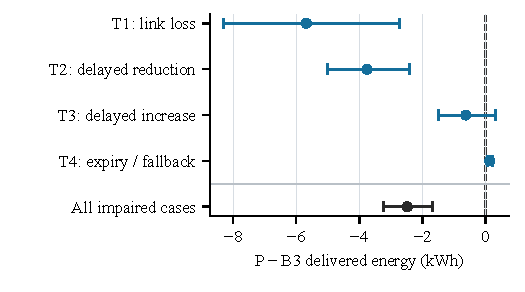
\includegraphics[width=\columnwidth]{paired_effects.pdf}
\caption{Paired supersession-minus-serialization energy differences. The 95\%
intervals resample 30 cohort blocks; each condition retains both loading levels.
Negative values favor B3.}
\label{fig:paired}
\end{figure}

P issues more commands than B3 (86.3 versus 68.1 per impaired episode) but
fewer queries (25.6 versus 49.1). Its integrated reserved-but-unused capacity
is smaller, 16.89 versus 22.19~kWh-equivalent, without greater delivered
energy. Reservation slack alone is therefore not a service objective.
Fig.~\ref{fig:trace} presents the prespecified median-effect T1 example,
selected across all 30 higher-loading cohorts. P delivers 9.43~kWh less
than B3 in this case.
R improves P's mean delivery to 481.9~kWh, but remains below B3; immediate
application evidence is not a service upper bound for a greedy scheduler.

\begin{figure}[t]
\centering
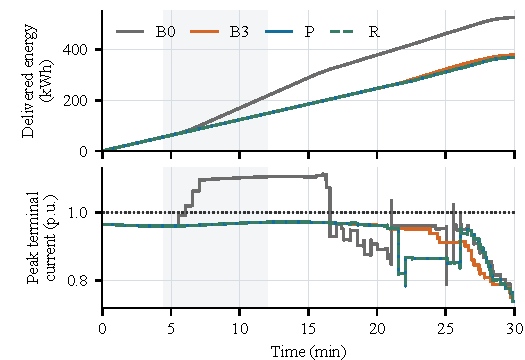
\includegraphics[width=\columnwidth]{representative_trace.pdf}
\caption{Median-effect T1 example (cohort 1011, loading center 1.0).
Curves show actual delivered energy and transformer terminal-phase loading.
The shaded interval spans the staggered link outages. All trace replays
reproduce their saved main-case metrics.}
\label{fig:trace}
\end{figure}

\subsection{Supplementary Retry Comparison}
Table~\ref{tab:retry} reports the separately frozen 960-episode follow-up. All four
implementations have zero electrical violations or cap-containment failures.
With retries enabled for both, P$_{\mathrm r}-$B3$_{\mathrm r}$ is
$-0.825$~kWh (95\% interval $[-1.137,-0.497]$), or $-0.17\%$.
On these same new cohorts, the query-only difference is $-2.406$~kWh.
Thus equal retry capability narrows the aggregate gap without establishing a
supersession service advantage. Retry-enabled P gains 0.400~kWh relative to
retry-enabled B3 in T1, while losing 3.370~kWh in T2.

\begin{table}[t]
\caption{Supplementary Retry Experiment: 240 Episodes per Policy.
Subscript r Denotes 60-s Same-Generation Retries.
Commands Include Retransmissions.}
\label{tab:retry}
\centering
% Post-review robustness experiment on new cohorts; initial primary analysis unchanged.
\begin{tabular}{lrrrr}
\hline
Policy & Energy & Unsafe & Commands & Queries \\
 & (kWh) & (/240) & (mean) & (mean) \\
\hline
B3 & 484.7 & 0 & 67.9 & 49.0 \\
P & 482.3 & 0 & 85.1 & 26.1 \\
B3$_{\mathrm{r}}$ & 483.0 & 0 & 93.6 & 12.9 \\
P$_{\mathrm{r}}$ & 482.2 & 0 & 93.6 & 10.0 \\
\hline
\end{tabular}

\end{table}

Retries are not guaranteed to improve this service metric: B3$_{\mathrm r}-$B3
is $-1.680$~kWh, while P$_{\mathrm r}-$P is $-0.099$~kWh with an interval
spanning zero. Retry attempts consume RPC opportunities otherwise available
for state queries and alter subsequent greedy reallocations. The measured
comparison supports the reservation accounting under both communication
strategies, without recommending either as an optimal scheduling policy.

\subsection{Sensitivity, Ablations, and Scope}
P and B3 remain violation-free in all 120 sensitivity cases per policy,
giving 420/420 when combined with their main cases. Longer evidence delay
can change service: at a 180-s certificate-delay extension, P$-$B3 is
$-3.15$~kWh with interval $[-5.56,-0.22]$. The 13-node checks also preserve
electrical feasibility; they do not establish topology-independent guarantees.
Across the 20 cases per ablation, omitting fallback accounting produces four
violating episodes and replacing locational admission with an aggregate budget
produces nine. Omitting pending-command accounting or crediting acceptance
produces no AC violation in these sampled cases. These null outcomes do not
establish that either omission is safe; they limit the empirical necessity
claim for those mechanisms. Both safeguards remain assumptions of the formal
result and are covered by execution-level regression tests.

On the recorded shared execution host, the median of episode-level median
filter times is 0.773~ms for P and 0.619~ms for B3; observed maxima are
37.88 and 15.28~ms. These exclude AC replay and communication, and are not
real-time implementation guarantees. Source, frozen scenarios, raw episode data,
analysis scripts, and editable SVG figures are available at
\url{https://github.com/asayghe1/ev-charging-cyber-resilient-recovery}.
Synthetic demand, fixed acceptance limits, static feeder controls, and the
trusted adapter restrict external validity. The implemented serialization
variant provides greater aggregate service in the primary study; supersession
is an option under the same reservations with condition-dependent service
effects. This comparison does not establish an optimal production recovery policy.


\section{Conclusion}
Execution-consistent reservations connect uncertain charging commands to feeder
capacity that can actually be reused. Under the stated adapter contract,
reserve-before-send, retained unresolved generations, and explicit expiry
fallback preserve containment and the selected affine feasibility rows.
The AC study finds no electrical violations for either reservation variant,
while serialization delivers slightly more energy overall than nonexpanding
supersession, including when both methods retry unresolved commands.
This separates the safety contribution of execution accounting
from the scheduling choice of when to replace a pending operation.
Deployment requires validating the adapter contract,
clock and tracking bounds, certificate integrity, and network-model accuracy on
physical chargers. Field charging traces and low-voltage network detail remain
necessary to assess operational generalization.

\section*{Acknowledgment}
OpenAI ChatGPT~\cite{openai2026chatgpt} was used to develop the exposition,
draft and revise the Abstract and Sections~I--VI, and generate and review
simulation, analysis, and figure code. The numerical results were obtained by
executing the supplied code; the figures plot those saved results.
\bibliographystyle{IEEEtran}
\bibliography{references}
\end{document}
